\chapter{随机抽样}
\section{Monte Carlo方法}
Monte Carlo方法是用随机数解决计算问题方法的统称。
\begin{method}{von Neumann舍选法}{}
	\begin{enumerate}
		\item 选取容易抽样的分布$h(x)$,使得曲线$Ch(x)$可以覆盖待抽样的分布$f(x)$;
		\item 从$h(x)$抽样得$x_i$;
		\item 从$\Unif(0,1)$抽样得$r_i$;
		\item 若$r_iCh(x_i)\leqslant f(x_i)$,则保留$x_i$,否则舍弃;
		\item 被接受的$x_i$序列,服从以$f(x)$为概率密度的分布;
		\item 使用$x_i$序列的算术平均,估算数学期望
	\end{enumerate}
	\begin{center}
		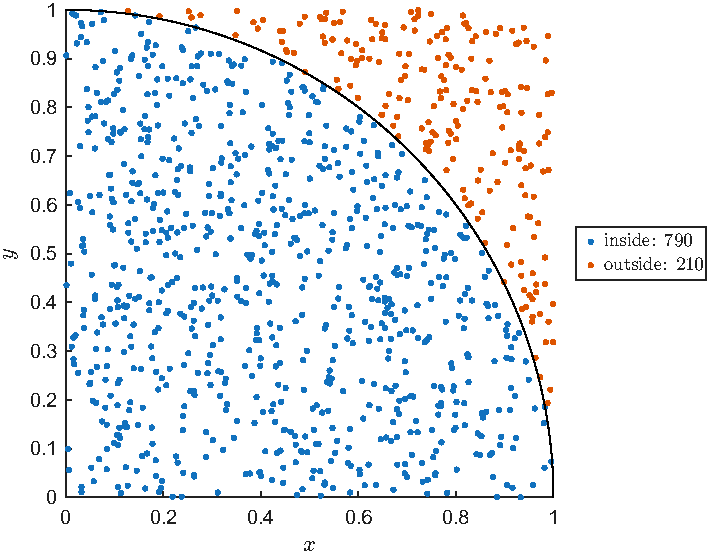
\includegraphics[width=0.6\linewidth]{figures/monte_carlo.pdf}
		\captionof{figure}{von Neumann舍选法计算$\pi\approx 4\times\frac{790}{1000}=3.16$}
		\label{fig:monte_carlo}
	\end{center}
\end{method}

\noindent
第4步是舍选法的关键步骤,但在高维问题中,无法知道$f(x)$的绝对数值,只知道相对值。

\begin{method}{Markov链法}{}
	把$f(x_i)$与上一个采样点$f(x_{i-1})$比较,
	以$\min\bigfkh{1,f(x_i)/f(x_{i-1})}$的概率接受$x_i$,否则令$x_i=x_{i-1}$。
\end{method}

\section{Bootstrap自助法}

\begin{quote}
	\textit{Why can not a man lift himself by pulling up on his bootstraps?}
\end{quote}
\begin{method}{bootstrap自助法}{}
	\begin{compactenum}
		\item 把样本看作总体的估计
		\item 从样本抽样(可放回),得到bootstrap样本
		\item 计算bootstrap样本的统计量
	\end{compactenum}
	\begin{center}
		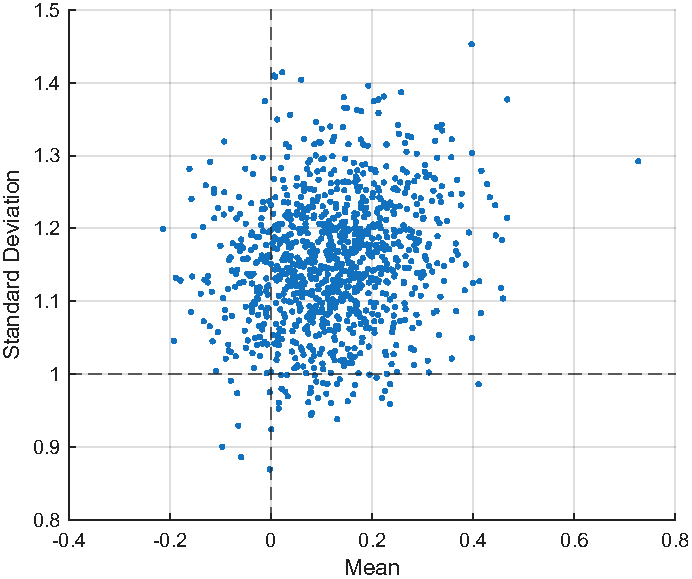
\includegraphics[width=0.6\linewidth]{figures/bootstrap.pdf}
		\captionof{figure}{对标准正态分布$\Norm(0,1)$的100个样本进行1000次bootstrap自助法得到的样本均值和方差分布}
		\label{fig:bootstrap}
	\end{center}
\end{method}
\begin{definition}{经验分布函数}{}
	$x_1,\ldots,x_n$是来自分布函数为$\CDF(x)$总体$X$的样本观察值。$X$的经验分布函数$\CDF_n(x)$定义为
	\begin{equation}
		\CDF_n(x)=\frac1n\sum_{i=1}^nI(x\geqslant x_i).
	\end{equation}
	用经验分布函数$\CDF_n$估计总体分布函数$\CDF$。
\end{definition}
从$\CDF_n$抽样可以看作是对样本$x_1,\ldots,x_n$进行可放回的重新抽样,称作bootstrap样本,记为$x_1^\ast,\ldots,$或$\bm x^\ast$。

使用一系列$\bm x^\ast$,得到相应的$\hat\theta_b^\ast=\hat\theta(\bm x_b^\ast)$。定义
\[
	\avg\theta^\ast=\frac1B\sum_{i=1}^B\hat\theta_b^\ast.
\]
为$\theta$的bootstrap估计。
\begin{theorem}{bootstrap中心极限定理}{bootstrap CLT}
	当总体$\CDF $换为经验分布$\CDF_n $时,$\E(\hat\theta)\to\avg\theta^\ast$,$\theta\to\hat\theta$
	\begin{equation}
		\avg\theta^\ast-\hat\theta\pto\E(\hat\theta)-\theta.
	\end{equation}
	收敛速度比正态分布CLT预测得更快,称为自助法的二次修正。
\end{theorem}
计算$\E_{\CDF_n}(\hat\theta)$需要考虑所有的$n^n$种重抽样可能性。计算量过大,改良为使用Monte Carlo方法近似从$ x_1, \ldots, x_n $进行随机重抽样